\documentclass[twocolumn]{article}
%\usepackage{natbib}
\usepackage[left=2cm,top=2.5cm,right=1.8cm,bottom=2.5cm,bindingoffset=0.0cm]{geometry}
\usepackage{graphicx}
\setlength\parindent{0pt}
\setlength{\columnsep}{30pt}
\usepackage{amsmath,amscd,amssymb}
\usepackage[justification=justified,singlelinecheck=false]{caption}
%\usepackage{algorithm}
%\usepackage[noend]{algpseudocode}
 \usepackage[linesnumbered,vlined ]{algorithm2e} 
\renewcommand{\thealgocf}{}

\makeatletter
\renewcommand{\@algocf@capt@plain}{above}% formerly {bottom}
\def\BState{\State\hskip-\ALG@thistlm}
\makeatother

\begin{document}
\twocolumn[{%
 \centering
 \LARGE  Estimating Stochastic Shortest Paths\\[1em]
 \large Michael W. Ramsey\\[3em]
}]

\bibliographystyle{ieeetr}
%\bibliographystyle{plain}

\begin{abstract}
We consider a special case of the Stochastic Shortest Path problem in which edge costs have a known distribution and we derive the induced shortest path distribution. This case often arises from situations where edge weights result from a noisy measurement or collection process. We model this case by introducing white noise to the edge weights of a standard weighted graph. Using the resulting stochastic graph we derive computational methods for the stochastic shortest paths distribution $p^*$. We present a new algorithm based on these methods, called Approximate Stochastic Paths (Asp). Preliminiary tests using the NetworkX Python library \cite{netx} suggest that Asp is faster and more accurate than the common Monte Carlo simulation-based approach \cite{frank_1969}.
\end{abstract}




\section{Introduction}
In applied problems, graph traversal costs often result from noisy measurement or collection processes, or result from an inherently stochastic cost. For example, a traveler on her daily commute may experiences different travel costs due to varying taffic levels, weather conditions, or incident levels such as work zones, accidents, and vehicle breakdowns. In this case, a road network model with stochastic edge weights provides a more realistic representation of a road network than a deterministic one.\\

This paper is organized as follows. Section 2 establishes prequisite definitions and results to formally define our problem. Next, in section 3  we present two methods for solving the problem. Section 4 discusses approximation methods for non-negative weights. Section 5 presents the Asp algorithm and provides test results. Section 6 discusses miscellaneous items. 




\section{Problem Definition}
Consider a weighted graph $G$ defined by triple $G = (V, E,C)$ where $V = {1, 2, . . . , n}$ is a set of nodes, $E$  is the edges subset of $V \times V$, and $C$ is the $n \times n$ matrix of edge weights or costs $c_{(i,j)} \in {{\mathbb R}}$. We discuss the non-negative case in the next section. Denote edges as $(i,j) \in E$ for $i,j \in V$.




\subsection{Stochastic Graphs}
We define the stochastic weighted graph induced by $G$ as $G^{\ast} = (V, E,C^{\ast} )$ with $C^{\ast}$  defined as the $n \times n$ matrix of edge cost distirbutions defined by 
\begin{gather}
Y_{(i,j)} = X_{(i,j)}c_{(i,j)} + c_{(i,j)}
\end{gather}

where $c_{(i,j)} \in C$ and $X_{(i,j)} \sim N(0,\sigma^{2})$  i.i.d. Thus we perturb the edge weights by a multiple of the original edge weight. The variance $\sigma^{2}$ of the white noise parameterizes the magnitude. \\

Note that by linearity of expected value and a basic property of variance we immediately obtain
\begin{gather}
Y_{(i,j)} \sim  N(c_{(i,j)},c_{(i,j)}^{2}\sigma^{2}).
\end{gather}


\subsection{Path Distributions}
Next we define a path $\pi_{i,j}$ as an ordered sequence of nodes $(v_{k})_{k=1}^{m}$ with $v_{1}=i$ and $v_{m}=j$  as source and destination nodes respectively and  $(v_{k},v_{k+1}) \in E,  \forall k$. A path is called simple if $v_{k} \ne v_{l}, \forall  k,l$. That is, there are no loops or cycles in the path. \\

Let $i,j \in V$ and define $\Pi_{i,j} =  \{ \pi_{i,j} \mid \pi_{i,j}  \text{ is simple}\}$. Then, for $\pi \in \Pi_{i,j}$ define
\begin{align}
Z_{\pi} & = \sum_{v_{k} \in \pi} Y_{(v_{k},v_{k+1})} \\
\hat{Z}_{\pi} & = \sum_{v_{k} \in \pi} {{\mathbb E}}(Y_{(v_{k},v_{k+1})}) \notag \\
& = \sum_{v_{k} \in \pi} c_{(v_{k},v_{k+1})}
\end{align}
as the stochastic and expected costs for path $\pi$ respectively. Note again, that by linearity of expectation and by a basic property of variance we get 
\begin{align}
 {{\mathbb E}}(Z_{\pi}) & =\hat{Z}_{\pi}  \notag \\
 & = \sum_{v_{k} \in \pi}  {{\mathbb E}}(Y_{(v_{k},v_{k+1})})   \notag \\
 & = \sum_{v_{k} \in \pi} c_{(v_{k},v_{k+1})}   \notag \\
\operatorname {Var}(Z_{\pi}) & = \sum_{v_{k} \in \pi} \operatorname {Var}(Y_{(v_{k},v_{k+1})})  \notag \\
& = \sum_{v_{k} \in \pi} c_{(v_{k},v_{k+1})}^{2}\sigma^{2}.  \notag
\end{align}

Therefore,
\begin{gather}
Z_{\pi} \sim N( \sum_{v_{k} \in \pi} c_{(v_{k},v_{k+1})} ,  \sum_{v_{k} \in \pi} c_{(v_{k},v_{k+1})}^{2}\sigma^{2}).
\end{gather}


\subsection{Stochastic Shortest Path}
Finally, we define the stochastic shortest path and the expected shortest path as
\begin{align}
\pi_{i,j}^{\ast}  & = \min_{\pi \in \Pi_{i,j}} Z_{\pi} \\
\hat{\pi}_{i,j}^{\ast} & = \min_{\pi \in \Pi_{i,j}} \hat{Z}_{\pi}.
\end{align}
Note that $\hat{\pi}_{i,j}^{\ast}$ can be computed directly from Dykstra's Algorithm (see \cite{dijkstra1959}) and that $\hat{\pi}_{i,j}^{\ast}$ is the mode of $\pi_{i,j}^{\ast}$.\\

We can now give our problem definition:
\begin{quote}
\fbox{%
\parbox{1\linewidth}{%
Given any weighted graph $G$ and $i,j \in V$, find $p^{*}(\pi_{i,j})=P(\pi_{i,j} = \pi^{\ast}_{i,j}), \forall \pi \in \Pi_{i,j}$.%
}%
}
\end{quote}

This provides the probability that $\pi_{i,j}$ is the shortest path between nodes $i,j$ for a random draw of edge weights from $G^{\ast}$ for any path $\pi_{i,j}$.




\section{Stochastic Path Distribution}

We present two approaches to computing the stochastic path distribution  $p^{*}$. The first solves for the distribution directly and requires numeric integration. The second estimates the distribution by sampling and aggregating the results. The best choice will depend on application details.



\subsection{Analytic Solution}
Given any weighted graph $G$, let $\pi \in \Pi_{i,j}$ for some $i,j \in V$ and $\Gamma_{\pi} = \Pi_{i,j}-\{\pi\}$. We can recast $P(\pi = \pi^{\ast})$ as $P(Z_{\pi}<W)$ where $W =  \min_{\gamma \in \Gamma_{\pi}} Z_{\gamma}$. By conditioning on $Z_{\pi}=s$ for some $s\in{{\mathbb R}}$ we obtain:
\begin{align}
P(Z_{\pi}=s, Z_{\pi}<W) & = P(Z_{\pi}=s)P(W>s \mid Z_{\pi}=s) \notag\\
& = P(Z_{\pi}=s)\prod_{\gamma \in \Gamma_{\pi}} P(Z_{\gamma}>s) \notag \\
& = P(Z_{\pi}=s)\prod_{\gamma \in \Gamma_{\pi}} (1-P(Z_{\gamma} \leq s)) \notag \\
& = f_{Z_{\pi}}(s)\prod_{\gamma \in \Gamma_{\pi}}(1-F(Z_{\gamma}(s))) \notag \\
& = f_{Z_{\pi}}(s)\prod_{\gamma \in \Gamma_{\pi}} SF(Z_{\gamma}(s))
\end{align}
since all the stochastic costs are independent; and where $f$ is the density for $ Z_{\pi}$ and $F$ and $SF$ are the cumulative distribution function and the  survival function for $Z_{\gamma}$.  $ Z_{\pi}$ and $Z_{\gamma}$ are distributed according to (5). \\

To determine $ P(Z_{\pi}<W)$ we simply need to integrate (8) over $s$:
\begin{align}
 P(Z_{\pi}<W) & = \int_{-\infty}^{\infty} P(Z_{\pi}=s, Z_{\pi}<W)  ds \notag \\
& = \int_{-\infty}^{\infty} f_{Z_{\pi}}(s)\prod_{\gamma \in \Gamma_{\pi}}SF(Z_{\gamma}(s))  ds
\end{align}

Therefore, given any simple path between any two nodes in a graph with noisy edge weights, (9) gives the probability it is the shortest path.


\subsection{Random Sample Solution}
Alternatively, by sampling each $Z_{\pi}$ directly using (5), we can calculate the frequency that $Z_{\pi}\leq\min_{\gamma \in \Gamma_{\pi}} Z_{\gamma}$ and use this to estimate  $p^{*}(\pi_{i,j})$, $ \forall \pi \in \Pi_{i,j}$.\\

Let $z_{\pi,k}$ be the $k$th random draw from  $Z_{\pi}$ out of $N \in{{\mathbb N}}$ many and $(z_{\pi,k})_{\pi \in \Pi_{i,j}}$ a random draw from all the $Z_{\pi}$. Define $m_{k}=\min_{\gamma \in \Gamma_{\pi}} z_{\gamma,k}$. Then the relative frequency that  $Z_{\pi}\leq\min_{\gamma \in \Gamma_{\pi}} Z_{\gamma}$ is computed as:
\begin{gather}
\omega_{N}(\pi = \pi^{\ast}) = \frac{ \sum_{k=1}^{N} \mathbf {1} _{{{\mathbb R}}^{+}}(m_{k}-z_{\pi,k})}{N}
\end{gather}
where $\mathbf {1} _{{{\mathbb R}}^{+}}\colon X\to \{0,1\}\,$ is the indicator function defined as:
\begin{gather}
{\displaystyle \mathbf {1} _{{{\mathbb R}}^{+}}(x)={\begin{cases}1&{\text{if }}x > 0,\\0&{\text{if }}x \leq 0.\end{cases}}} \notag
\end{gather}
Therefore, by the Law of Large Numbers, as $ N \rightarrow \infty$:
\begin{gather}
\omega_{N}(\pi = \pi^{\ast})\longrightarrow P(\pi = \pi^{\ast})
\end{gather}
where $P(\pi = \pi^{\ast}) = {{\mathbb E}}( {1} _{{{\mathbb R}}^{+}}(m_{k}-z_{\pi,k}))$.




\section{Non-Negative Weights}
Often, in applied settings, negative edge weights do not have a meaningful interpretation. Consider time or distance costs. In this case we apply the truncated normal distribution. However, to reproduce our results above we need to know the effect of scaling, shifting, and summing truncated normal random variables. 


\subsection{Truncated Normal Distribution}
The Truncated Normal Distribution is defined in two steps: (1) select parameters $\mu$ and $\sigma^{2}$ for a parent normal random variable $\phi \sim N(\mu,\sigma^{2})$ with CDF $\Phi$ and (2) select a truncation range $(a,b)$.  The truncated normal PDF $\psi(\mu,\sigma^{2},a,b;x)$ is defined as:
\begin{gather}
\psi(\mu ,\sigma ,a,b;x)={\frac {{\frac {1}{\sigma }}\phi ({\frac {x-\mu }{\sigma }})}{\Phi ({\frac {b-\mu }{\sigma }})-\Phi ({\frac {a-\mu }{\sigma }})}} \notag
\end{gather}
for $a \leq x\leq b$ and $0$ elsewhere. If $X$ has PDF $\psi(x;\mu ,\sigma^{2},a,b)$ we say $X \sim TN(\mu ,\sigma^{2})$ over $(a,b)$.\\

Note that the parameters $\mu$ and $\sigma^{2}$ are the mean and variance of the parent normal distribution, not of the truncated normal PDF itself. These are more complicated. Let $X \sim TN(\mu ,\sigma^{2})$ over $ (a,b)$, $\alpha =(a-\mu )/\sigma$, and $\beta =(b-\mu )/\sigma$. Then
\begin{gather}
{{\mathbb E}} (X) = \mu - \sigma \Delta_{0} \notag \\
\operatorname {Var}(X)= \sigma^{2}\left[1 - \Delta_{1}-\Delta_{0}^{2}\right] \notag
\end{gather} \\
where $\Delta_{k} = {\frac {\beta^{k} \phi (\beta )-\alpha^{k} \phi (\alpha)}{\Phi (\beta )-\Phi (\alpha )}}$. \\

By integrating $\phi$ appropriately, the truncated normal CDF is

$$\Psi(\mu ,\sigma ,a,b;x)={\begin{cases}0&{\text{if }} x \leq a,\\{\frac{\Phi ({\frac {x-\mu }{\sigma }})-\Phi ({\frac {a-\mu }{\sigma }})}{\Phi ({\frac {b-\mu }{\sigma }})-\Phi ({\frac {a-\mu }{\sigma }})}}&{\text{if }} a < x < b,\\1&{\text{if }} x \geq b.\end{cases}}$$


\subsection{Transformations}
Suppose $X \sim TN(\mu ,\sigma^{2})$ over $(a,b)$ and $c,d \in {{\mathbb R}}$. Then for $Y= cX+d$ we have
\begin{gather}
Y \sim TN(c\mu+d ,d^{2}\sigma^{2}) \\
\text{over }(ca+d,cb+d) \notag
\end{gather} 
 
In general, summing truncated normal random variables does not necessarily produce another truncated normal random variable. Fortunately though, this sum can be approximated by a truncated normal in the case where the summands are truncated symmetrically about their means (see \cite{eng}). \\

Let $X_{k} \sim TN(\mu_{k}  ,\sigma^{2}_{k})$ over $(a_{k} ,b_{k})$ for $k=1,2,\ldots n$ such that $\frac{b_{k}+a_{k}}{2} = \mu_{k}$. Then we can approximate the distribution of $Y=\sum_{k=1}^{n} X_{k} $ by
\begin{gather}
Y \approx TN(\sum_{k=1}^{n}{\mu_{k}} ,\sum_{k=1}^{n}\sigma_{k}^{2}) \\
\text{over } (\sum_{k=1}^{n} a_{k}, \sum_{k=1}^{n} b_{k}). \notag
\end{gather} 


\subsection{Stochastic Path Distribution}
We can use (12) and (13) to retrace the steps in  Section 2 for the truncated normal distribution. \\

Define the truncated stochastic weighted graph induced by $G$ as $G^{\ast}_{a,b} = (V, E,C^{\ast} )$ with $C^{\ast}$  defined as the $n \times n$ matrix of edge cost distirbutions defined by 
\begin{gather}
Y_{(i,j)} = X_{(i,j)}c_{(i,j)} + c_{(i,j)} 
\end{gather}

where $c_{(i,j)} \in C$ and $X_{(i,j)} \sim TN(0,\sigma^{2})$ over $(-1,1)$ i.i.d. Thus we perturb the edge weights by a percent of the original edge weight, but since $-1 \leq X_{(i,j)} \leq 1$, then $Y \geq 0$.\\

Applying (12) to (14) we immediatly obtain:
\begin{gather}
Y_{(i,j)} \sim  TN(c_{(i,j)},c_{(i,j)}^{2}\sigma^{2})\notag\\
\text{over } (0,2c_{(i,j)}). \notag
\end{gather}

Let $\Pi_{i,j}$ be defined as in Section 2. Then, for $\pi \in \Pi_{i,j}$ define
\begin{align}
Z_{\pi} & = \sum_{v_{k} \in \pi} Y_{(v_{k},v_{k+1})}.\notag
\end{align}
Next we can apply (14) to $Z_{\pi}$ to get:
\begin{gather}
Z_{\pi} \approx TN( \sum_{v_{k} \in \pi} c_{(v_{k},v_{k+1})} ,  \sum_{v_{k} \in \pi} c_{(v_{k},v_{k+1})}^{2}\sigma^{2}) \\
\text{over } (0,\sum_{v_{k} \in \pi}  2c_{(v_{k},v_{k+1})}). \notag
\end{gather}
The results of Section 3 then follow analogously substituting (15) for (5).


\subsection{Contribution}
In addition to generating the performance improvements provided by Asp, detailed in the next section, the above results provide several benefits.
\begin{itemize}
\item Numerically soving the integral in (9) provides a accurate, well studied benchmark for validating code and algorithms.
\item Detailing path distributions, as in (5), allows for more sophisticated modeling of path selection decision making. For example, depending on the utility function under consideration, path selection can use (5) to pick the path with the least risk rather than lowest expected cost.
\end{itemize}




\section{Computing  Distributions}
Next, we detail a new algorithm, called Approximate Stochastic Paths (Asp), that combines the above results with a standard $k$-shortest paths algorithm. Preliminiary tests using the  NetworkX Python library suggest that Asp is faster and more accurate than the common simulation-based approach (see \cite{frank_1969}).


\subsection{The Asp Algorithm}
Asp estimates $p^{*}(\pi_{i,j})$ for any nodes $i,j$ in a weighted graph $G$ in two main steps. The first step, denoted SHORT, uses the top $k$ shortest paths (kSP) between nodes $i,j$ using NetworkX's version of Yen's algorithm (see \cite{netx}, \cite{Yen1971})on the deterministic edge weights $c_{(v_{k},v_{k+1})}$, $v_{k} \in \pi$, from $G$. The second step, denoted FREQ, estimates $\omega_{N}(\pi = \pi^{\ast})$ using equation (10). Asp automatically estimates the two required parameters, $k$ and $N$, using user provided tolerances.\\



\begin{algorithm}
\SetKwFunction{algo}{algo}\SetKwFunction{proc}{proc}
\DontPrintSemicolon

\KwData{$G = (V, E,C)$, $i,j$, $\sigma$, $b_{k}$, $b_{N}$, $t_{k}$, $t_{N}$, $\epsilon$.}
\KwResult{$\{ (\omega_{N}(\pi = \pi^{\ast}),(v_{k},v_{k+1})) \mid v_{k} \in \pi \subset \Pi_{i,j} \}$.}

\Begin{
$g =$  kSP($G, i, j$)\;

\SetKwProg{myproc}{SHORT($g$, $b_{k}$, $t_{k}$)}{}{}
\myproc{}{
$\Pi = \emptyset$\;
\Begin{
$p = 1$\; 
\While{$p > t_{k}$}{
$\Pi = \Pi \cup g(b_{k})$\;
$\gamma = $ First($\Pi$)\;
$\pi  = $ Last($\Pi$)\;
$\bar{\mu} =  \sum_{\pi} c_{(v_{k},v_{k+1})} - \sum_{ \gamma} c_{(v_{k},v_{k+1})}$ \;
$\bar{\sigma}^{2} = \sum_{\pi} c_{(v_{k},v_{k+1})}^{2}\sigma^{2} + \sum_{\gamma} c_{(v_{k},v_{k+1})}^{2}\sigma^{2}$ \;
$Z_{\gamma} - Z_{\pi} = TN(\bar{\mu}, \bar{\sigma}^{2})$ \;
$p = SF_{Z_{\gamma} - Z_{\pi}}(0)$\;
}}\KwRet $\Pi$}


\SetKwProg{myproc}{FREQ($\Pi$, $\sigma$, $b_{N}$, $t_{N}$, $\epsilon$)}{}{}
\myproc{}{

\Begin{
$\Omega = \emptyset$\;
\For{$\pi \in \Pi$}{
$\bar{\mu} =  \sum_{\pi} c_{(v_{k},v_{k+1})}$ \;
$\bar{\sigma}^{2} = \sum_{\pi} c_{(v_{k},v_{k+1})}^{2}\sigma^{2}$ \;
$Z_{\pi} = TN( \bar{\mu}, \bar{\sigma}^{2} )$}

\For{$\pi \in \Pi$}{
$N= b_{N}$ \;
$ ((z_{\pi,k})_{\pi \in \Pi}) = $DRAW($n, (Z_{\pi})_{\pi \in \Pi}$) \;
$\Gamma_{\pi} = \Pi-\{\pi\}$ \;
$m_{k}=\min_{\gamma \in \Gamma_{\pi}} z_{\gamma,k}$. \;
$\omega_{N} = \frac{ \sum_{k=1}^{N} \mathbf {1} _{{{\mathbb R}}^{+}}(m_{k}-z_{\pi,k})}{N}$ \;
$\delta_{N} = \lvert  \omega_N - \omega_{N-\epsilon} \rvert$ \;
\While{$\delta_{N} > t_{N}$}{
$N = N + b_{N}$\;
$ ((z_{\pi,k})_{\pi \in \Pi}) = $DRAW($n, (Z_{\pi})_{\pi \in \Pi}$) \;
$\Gamma_{\pi} = \Pi-\{\pi\}$ \;
$m_{k}=\min_{\gamma \in \Gamma_{\pi}} z_{\gamma,k}$. \;
$\omega_{N} = \frac{ \sum_{k=1}^{N} \mathbf {1} _{{{\mathbb R}}^{+}}(m_{k}-z_{\pi,k})}{N}$ \;
$\delta_{N} = \lvert  \omega_N - \omega_{N-\epsilon} \rvert$ \;
}
$\Omega = \Omega \cup (\omega_{N}, \pi)$}

}return $\Omega$\;}return FREQ(SHORT( $g$, $b_{k}$, $t_{k}$ ), $\sigma$, $b_{N}$, $t_{N}$, $\epsilon$) 
}
\caption{Asp - Truncated Normal Version \label{asp}}
\end{algorithm}


Yen's algorithm computes the $k$ shortest simple paths for a graph with non-negative edge cost. The algorithm employs any shortest path algorithm to find the best path, then proceeds to find $k-1$ deviations of the best path. The  NetworkX implementation uses a bi-directional Dijkstra's algorithm and returns a Python generator allowing iterative queries for the next shortest path. \\

Asp uses the Python generator's efficiency to retrieve shortest paths in batches of size $b_{k}$ and stops when the probability, that the last path retrieved would ever be shorter than the first retrieved, is below a user provided threshold $t_{k}$.  More formally, the stopping condition is $P(Z_{\pi} < Z_{\gamma}) < t_{k} $ where $\pi$  and $\gamma$ are the first and last path retrieved respectively. This works because $P(Z_{\pi} < Z_{\gamma})$ is an upper bound on $P(Z_{\pi}<W)$ where $W =  \min_{\gamma \in \Gamma_{\pi}} Z_{\gamma}$ and can be computed quickly as:
\begin{align}
P(Z_{\pi} < Z_{\gamma}) &=  P(Z_{\pi} - Z_{\gamma}) < 0 \notag \\ 
&= 1 - P(Z_{\gamma} - Z_{\pi}) \leq 0 \notag \\ 
&= 1 - CDF_{Z_{\gamma} - Z_{\pi}}(0) \notag \\ 
&= SF_{Z_{\gamma} - Z_{\pi}}(0) \notag
\end{align}

where
\begin{align}
Z_{\gamma} - Z_{\pi} \sim N(\mu_{\gamma}-\mu_{\pi},\sigma_{\gamma}^{2}+\sigma_{\pi}^{2}) \notag
\end{align}
or 
where
\begin{gather}
Z_{\gamma} - Z_{\pi} \approx TN(\mu_{\gamma}-\mu_{\pi},\sigma_{\gamma}^{2}+\sigma_{\pi}^{2}) \notag \\
\text{over } (-2\mu_{k},2\mu_{k}) \notag
\end{gather}
depending on whether the weights must be non-negative or not.\\

To select the number $N$ of samples to draw from $Z_{\pi}$, Asp again works in batchs of size $b_{N}$ and stops when the marginal change $\delta_{N}$ in $\omega_N$ falls below a provided threshold  $t_{N}$. If the marginal change is not below $t_{N}$, it draws $b_{N}$ more, recomputes, tests, and repeats until the threshold is met. Asp computes the marginal change as $\delta_{N} = \lvert  \omega_n - \omega_{n-\epsilon} \rvert$ for some user provided $\epsilon$ and for $n$ equal to $b_{N}$ times the number of completed iterations.


\subsection{Simulating $p^{*}$}
The popularity of estimating $p^{*}$ via simulation comes from its relative simplicity: for some number of iterations $i = 1 \dots n$, the algorithm computes $f_N$ by running Dykstra's algorithm on $G^{*}_{i}$, where $G^{*}_{i}$ is newly generated from $G$ in each iteration.




\subsection{Experimental Results}
As a preliminary test of Asp, we compare its performace to Monte Carlo simulation on a series of small synthetic graphs where we control the number and length of paths between two points. Each test graph consists of a set number $m$ of disjoint paths with random length and weights drawn uniformly from $(10,15)$ and $(0,10)$ respectively. For this study, we used $m = 2 \dots 10$. \\

To evaluate Asp's accuracy in the absence of groundtruth, we exploit the fact that the simulation estimate of $p^{*}$ should improve as the number of iterations increases. If Asp is more accurate than the simulation estimates, then as we increase the number of iterations, the simulation estimate should approach Asp's estimate. Therefore, this experiment records the difference between Asp's estimates and the simulated estimates, along with their respective computation times. \\

In this experiment we performed three trials and averaged the results for each test graph. Each trial consisted of running Asp and the simulation algorithm on each test graph. We ran the simuation for each of $10^{2}$, $10^{3}$, and $10^{4}$ iterations. For each trial we recorded the average difference between Asp's estimates and the simulated estimates, along with their respective computation times. We also set $\sigma = .2$ because simulation took too many iterations and too much time to achieve reasonable probability estimates.\\


The experimental results,  shown in Figure 1 and Figure 2, indicate that Asp is both faster and it's estimate is more accurate than the simulations. As the number of simulation runs increases, the simulation estimate deviates proportionatly less from the Asp estimate. Given that the similation estimate should be getting better as the iteration runs increase, we conclude Asp is more accurate. Spot checking the results and one-off comparisons to numerical integration estimates based on (9) also supports this conclusion. Further, the computation times of Asp remains constant as the number of paths increases, whereas simulation times increase significantly.

\begin{figure}
\centering  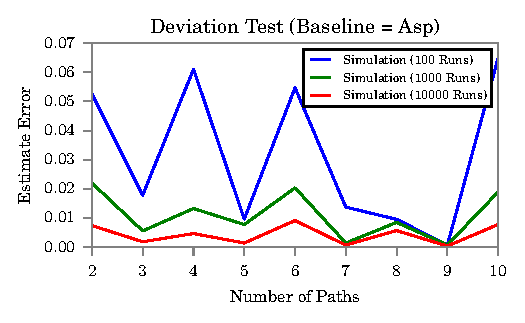
\includegraphics[width=\linewidth]{simulation_convergence.pdf}
  \caption{Deviation of simulation estimates from Asp's estimate for each of $10^{2}$, $10^{3}$, and $10^{4}$ iterations. }
\end{figure}


\begin{figure}
\centering  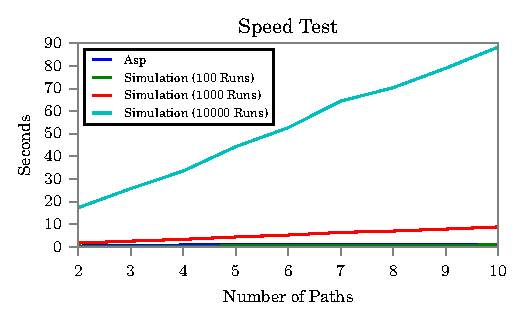
\includegraphics[width=\linewidth]{simulation_times.pdf}
  \caption{Computing times of Asp and  simulation estimates for each of $10^{2}$, $10^{3}$, and $10^{4}$ iterations. }
\end{figure}


\section{Discussion}

\subsection{Caveats}
It is important to stress the limitations of this experiement and note that futher research is required. Experimental results could vary depending on $\sigma$, Asp paramenter choices, software implementations, or graph properties. We did run one variation of the study using kSP as input into the simulation to help prune the computation, but found little performance improvement.

\subsection{Edge Traversal Probability}
Extending estimates for $p^{*}$ to edge traversal probabilities arises naturally in the simulation algorithm since edge traversal counts can be easily obtained from path traversals. Such accounting does not come easily with Asp. However, the probability of an edge being traversed can be computed from the probabilities of the paths containing it. \\

For example, suppose there is a distribution over the nodes giving the probability $P( (i,j) = (s,e))$ each pair of nodes would be selected as endpoints $(s,e)$. Then, given any edge $(u,v)$, the probability $(u,v)$ is traversed could be defined as:
\begin{gather}
P( (u,v) \text{ traversed } ) = \sum_{(u,v) \in \pi_{i,j}} p^{*}_{\pi_{i,j}} P( (i,j) = (s,e))) \notag
\end{gather}


\subsection{Other Distributions}
Reproducing our resutls only requires knowing the effect of scaling, shifting, and summing a random variable for any distribution. Therefore, both our derivations and Asp should be extendable to a wide range of edge cost noise models.

\subsection{Other Decision Models}
This paper focuses on the the global shortest path using a single decision criteria - edge weights. There are many situations where path selection is based on local information, only the next path, or multiple criteria, such as total edge cost and the number to nodes traversed. Possible extentions include investigating multiobjective models and short-sighted decision making (see \cite{multiobj}, \cite{hall_1986}).


\section{Conclusion}
We considered a special case of the Stochastic Shortest Path problem in which edge costs have a known distribution and we derive the induced shortest path distribution. We induced a stochastic weighted graph from a standard weighted graph by introducing white noise to the edge weights. Using this graph we derived computational methods for the stochastic shortest paths distribution $p^*$ and presented a new algorithm based on these methods, called Approximate Stochastic Paths (Asp). \\

Our experimental results indicate that Asp is both faster and it's estimate is more accurate than the more common Monte Carlo simulation approach. As the number of simulation runs increases, the simulation estimate deviates proportionatly less from the Asp estimate. Given that the similation estimate should be getting better as the iteration runs increase, we conclude Asp is more accurate. Spot checking the results and one-off comparisons to numerical integration estimates based on (9) also supports this conclusion. Further, the computation times of Asp remains constant as the number of paths increases, whereas simulation times increase significantly. \\

In addition to generating these performance improvements, our results provide several benefits. First, Numerically soving the integral in (9) provides a accurate, well studied benchmark for validating code and algorithms. Second, detailing path distributions, as in (5), allows for more sophisticated modeling of path selection decision making. For example, depending on the utility function under consideration, path selection can use (5) to pick the path with the least risk rather than lowest expected cost.



\bibliography{ssp}

\end{document}
